\subsubsubsubsection{Bus Stop}
\begin{figure}[h]
\centering
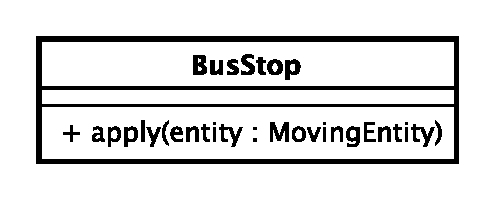
\includegraphics[scale=0.6,keepaspectratio]{images/solution/bus_stop.eps}
\caption{App::Passive::BusStop}
\label{fig:sd-app-bus_stop}
\end{figure}
\FloatBarrier
\begin{itemize}
  \item \textbf{Description} \\
It implements the bus stop road sign. It queries a pedestrian to know if it wants to wait for the bus.
  \item \textbf{Operation}
  \begin{itemize} 
  \item \texttt{+ apply(entity: Pedestrian)} \\
Notifies the pedestrian to know if it wants to wait for the bus. If the pedestrian wants
to take the bus then a timeout is registered for the pedestrian.
  \end{itemize}
\end{itemize}
